% SPDX-License-Identifier: CC-BY-SA-4.0
% Author: Matthieu Perrin
% Part: 
% Section: 
% Sub-section: 
% Frame: 

\begingroup

\begin{frame}{Application du lemme d'Arden}
  \small 
  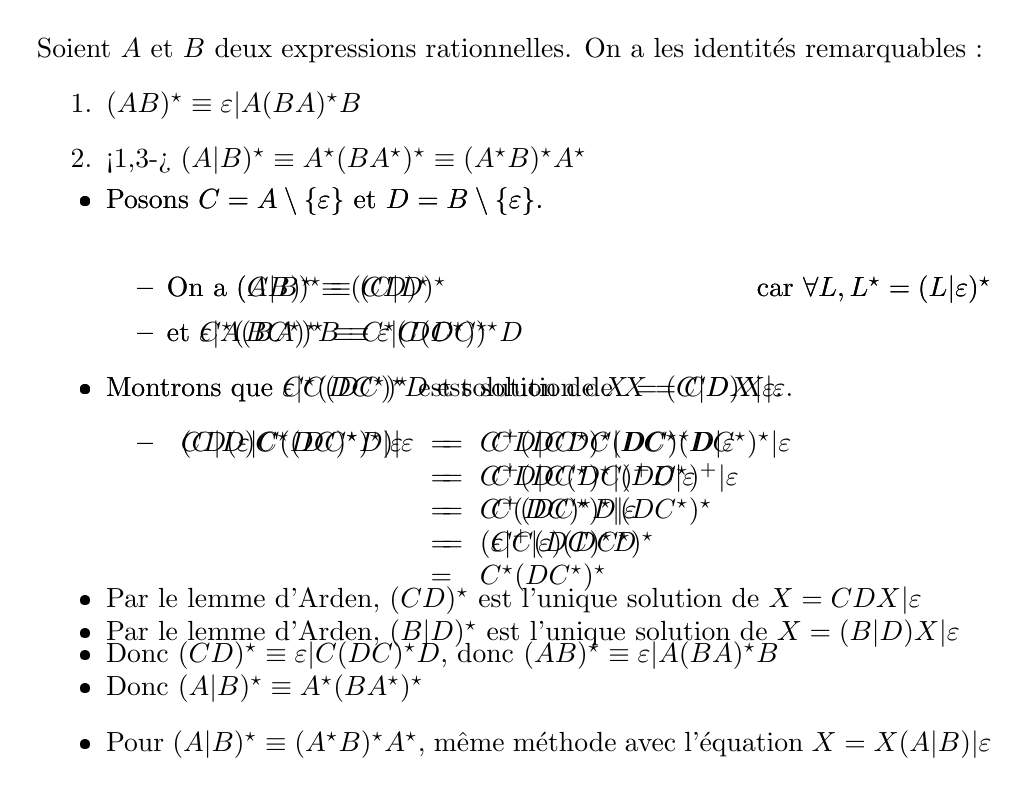
\begin{tikzpicture}

    \draw (10,10) node[below]{\begin{minipage}{\textwidth}
        Soient $A$ et $B$ deux expressions rationnelles. On a les identités remarquables : 
        \begin{enumerate}
        \item       \structure{$(AB)^\star \equiv \varepsilon | A(BA)^\star B$}
        \item<1,3-> \structure{$(A | B)^\star \equiv A^\star (B A^\star)^\star  \equiv (A^\star B)^\star A^\star$}
        \end{enumerate}
    \end{minipage}};

    \draw<2|handout:1> (10,8.1) node[below]{\begin{minipage}{\textwidth}
        \begin{itemize}
        \item Posons $C = A \setminus \{\varepsilon\}$ et $D = B \setminus \{\varepsilon\}$.\\
          \begin{itemize}
          \item On a $(A B)^\star \equiv (C D)^\star$  \hspace\fill car $\forall L, L^\star = (L | \varepsilon)^\star$
          \item et $\varepsilon  | A (B A)^\star B \equiv \varepsilon | C (D C)^\star D$
          \end{itemize}
        \item Montrons que $\varepsilon | C (D C)^\star D$ est solution de $X = CD X | \varepsilon$.
          \begin{itemize}
          \item $\begin{array}[t]{rclrcl}
            \structure{CD (\example{\varepsilon | C (D C)^\star D}) | \varepsilon}
            & = & CD | CD C (D C)^\star D | \varepsilon\\
            & = & CD | C (D C)^+ D | \varepsilon\\
            & = & C (D C)^\star D | \varepsilon\\
            & = & \example{\varepsilon | C (D C)^\star D}\\
          \end{array}
            $
          \end{itemize}
        \item Par le lemme d'Arden, $(CD)^\star$ est \alert{l'unique} solution de $X = CD X | \varepsilon$
        \item Donc $(CD)^\star \equiv \varepsilon | C (D C)^\star D$, donc $(AB)^\star \equiv \varepsilon | A (BA)^\star B$
        \end{itemize}
    \end{minipage}};

    \uncover<3-|handout:2>{
      \draw (10,8.1) node[below]{\begin{minipage}{\textwidth}
          \begin{itemize}
          \item Posons $C = A \setminus \{\varepsilon\}$ et $D = B \setminus \{\varepsilon\}$.\\
            \begin{itemize}
            \item On a $(C | B)^\star \equiv (C | D)^\star$ \hspace\fill car $\forall L, L^\star = (L | \varepsilon)^\star$
            \item et $C^\star (B C^\star)^\star \equiv C^\star (D C^\star)^\star$
            \end{itemize}
          \item Montrons que $C^\star (DC^\star)^\star$ est solution de $X = (C|D) X | \varepsilon$.
            \begin{itemize}
            \item $\begin{array}[t]{rclrcl}
              \structure{(C|D) \example{C^\star (DC^\star)^\star} | \varepsilon}
              & = & C^+ (DC^\star)^\star | D C^\star (DC^\star)^\star | \varepsilon\\
              & = & C^+ (DC^\star)^\star | (DC^\star)^+ | \varepsilon\\
              & = & C^+ (DC^\star)^\star | (DC^\star)^\star\\
              & = & (C^+|\varepsilon) (DC^\star)^\star\\
              & = & \example{C^\star (DC^\star)^\star}\\
            \end{array}
              $
            \end{itemize}
          \item Par le lemme d'Arden, $(B |D)^\star$ est \alert{l'unique} solution de $X = (B|D) X | \varepsilon$
          \item Donc $(A | B)^\star \equiv A^\star (B A^\star)^\star$
          \item Pour $(A | B)^\star \equiv (A^\star B)^\star A^\star$, même méthode avec l'équation $X = X (A|B) | \varepsilon$
          \end{itemize}
      \end{minipage}};
    }    
  \end{tikzpicture}
\end{frame}


\endgroup
